%%%%%%%%%%%%%%%%%%%%%%%%%%%%%%%%%%%%%%%%%
% Beamer Presentation
% LaTeX Template
% Version 1.0 (10/11/12)
%
% This template has been downloaded from:
% http://www.LaTeXTemplates.com
%
% License:
% CC BY-NC-SA 3.0 (http://creativecommons.org/licenses/by-nc-sa/3.0/)
%
%%%%%%%%%%%%%%%%%%%%%%%%%%%%%%%%%%%%%%%%%

%----------------------------------------------------------------------------------------
%	PACKAGES AND THEMES
%----------------------------------------------------------------------------------------

\documentclass{beamer}

\mode<presentation> {

% The Beamer class comes with a number of default slide themes
% which change the colors and layouts of slides. Below this is a list
% of all the themes, uncomment each in turn to see what they look like.

%--------------------------------------------------------------------------------------------------------
%--------------------------------------------------------------------------------------------------------
%\usetheme{default} % Nothing: all white, navigation icons
%--------------------------------------------------------------------------------------------------------
%\usetheme{AnnArbor} % Horizontal with columns, top section and subsection, bottom Name, short title date and slide number out of, Blue yellow
%\usetheme{CambridgeUS} % Red grey
%\usetheme{Boadilla} % As above, but only bottom part, blue tones
%\usetheme{Madrid} % No first bar top, only title bar, dark blue themes
%--------------------------------------------------------------------------------------------------------
%\usetheme{Antibes} % Black Blue, Horizontal, only top, Short title, section and subsection tree
%\usetheme{Montpellier} % No real blocks, top bar is between light blue lines, very white
%\usetheme{JuanLesPins} % Very the same, no tree icons but indentation
%--------------------------------------------------------------------------------------------------------
%\usetheme{Bergen} % Thick Bar left with structure elements (icons, stuff)
%--------------------------------------------------------------------------------------------------------
%\usetheme{Berkeley} % Bar left and top, top slide title, left, Title, name and toc
%\usetheme{PaloAlto} % As Berkely minor changes, White on blue in bars
%\usetheme{Goettingen} % Bar right, with info as above, no top bar, light blue theme
%\usetheme{Hannover} % Same as Goettingen, bar left
%\usetheme{Marburg} % Bar with gradient from black to blue
%--------------------------------------------------------------------------------------------------------
%\usetheme{Berlin} % Horizontal 3 bars top, Sections with # of slides icon and progress marker, 2nd bar subsection, Slide title in 3rd bar, Bottom 2 bars, Name and institute, last bar short title, White on shades of blue
%\usetheme{Ilmenau} % almost identical to Berlin
%\usetheme{Szeged} % Very plain, boxes between blue lines, Title not in box, bottom 1 box, Short title and institute 
%\usetheme{Darmstadt} % White on blue/black, as above but only top
%\usetheme{Dresden} % As Berlin, but Slide Title isn't an own bar
%\usetheme{Frankfurt} % as Darmstadt, no 2nd bar
\usetheme{Singapore} % Very simple, only some blue shading in on top as box, Sections with Progress marker
%--------------------------------------------------------------------------------------------------------
%--------------------------------------------------------------------------------------------------------

%\usetheme{Copenhagen} % Blue/Black, Bar with 2 columns, left sections with highlight, right subsections with highlight,Big bar with slide title,  bottom bar with 2 columns, Name and then Short title
%\usetheme{Warsaw} % As Copenhagen, Slide title bar fades form blue to black
%\usetheme{Luebeck} % Very much like Copenhagen, minor alignment changes
%\usetheme{Malmoe} % Slide title not in bar
%--------------------------------------------------------------------------------------------------------
%\usetheme{Pittsburgh} % Very Plain, only Slide title in blue on top, right flushed
%\usetheme{Rochester} % As above, Slide title in white on blue block
%--------------------------------------------------------------------------------------------------------
%--------------------------------------------------------------------------------------------------------

% As well as themes, the Beamer class has a number of color themes
% for any slide theme. Uncomment each of these in turn to see how it
% changes the colors of your current slide theme.

%\usecolortheme{albatross}
%\usecolortheme{beaver}
%\usecolortheme{beetle}
%\usecolortheme{crane}
%\usecolortheme{dolphin}
%\usecolortheme{dove}
%\usecolortheme{fly}
%\usecolortheme{lily}
%\usecolortheme{orchid}
%\usecolortheme{rose}
%\usecolortheme{seagull}
%\usecolortheme{seahorse}
%\usecolortheme{whale}
%\usecolortheme{wolverine}

%\setbeamertemplate{footline} % To remove the footer line in all slides uncomment this line
%\setbeamertemplate{footline}[page number] % To replace the footer line in all slides with a simple slide count uncomment this line

%\setbeamertemplate{navigation symbols}{} % To remove the navigation symbols from the bottom of all slides uncomment this line
\setbeameroption{show notes}
}

\usepackage{graphicx} % Allows including images
\usepackage{booktabs} % Allows the use of \toprule, \midrule and \bottomrule in tables
\usepackage{enumitem}
\usepackage{tikz}
\usetikzlibrary{shapes.geometric, arrows}
\usetikzlibrary{mindmap, backgrounds}

\tikzstyle{decision} = [diamond, minimum width=3cm, minimum height=1cm, text centered, draw=black, fill=green!30]
\tikzstyle{process} = [rectangle, minimum width=3cm, minimum height=1cm, text centered, draw=black, fill=orange!30]
\tikzstyle{startstop} = [rectangle, rounded corners, minimum width=3cm, minimum height=1cm,text centered, draw=black, fill=red!30]
\tikzstyle{io} = [trapezium, trapezium left angle=70, trapezium right angle=110, minimum width=3cm, minimum height=1cm, text centered, draw=black, fill=blue!30]
\tikzstyle{arrow} = [thick,->,>=stealth]
 % ExercisesH, ExerciseswNotesH, ExercisesHandoutH, NotesH
% (= SlidesH, SlideswNotesH, HandoutH, NotesH, Slides2ScreensH,

\graphicspath{{../../../images/Exercises/}} % Location of the slide background and figure files

%----------------------------------------------------------------------------------------
%	TITLE PAGE
%----------------------------------------------------------------------------------------

\title{Handstand and preliminary exercises} % The short title appears at the bottom of every slide, the full title is only on the title page


\author{Raphael Nussbaum} % Your name
\institute[Stress Regulation] % Your institution as it will appear on the bottom of every slide, may be shorthand to save space
{
AJ Tutoring Nerd Fest \\
%Stress regulation YouTube channel \\ % Your institution for the title page
\medskip
\textit{raphaelnussbaum@ajtutoring.com}
%regulate.stress@gmail.com} % Your email address
}
\date{\today} % Date, can be changed to a custom date



\begin{document}

\begin{frame}
\titlepage % Print the title page as the first slide
\end{frame}



%-------------------------------------------------------------------
\begin{frame}
\frametitle{Starting position}
\hypertarget{hemi}{}
\begin{columns}[c] % The "c" option specifies centered vertical alignment while the "t" option is used for top vertical alignment

\column{0.7\textwidth} % Left column and width
%	\begin{figure}
	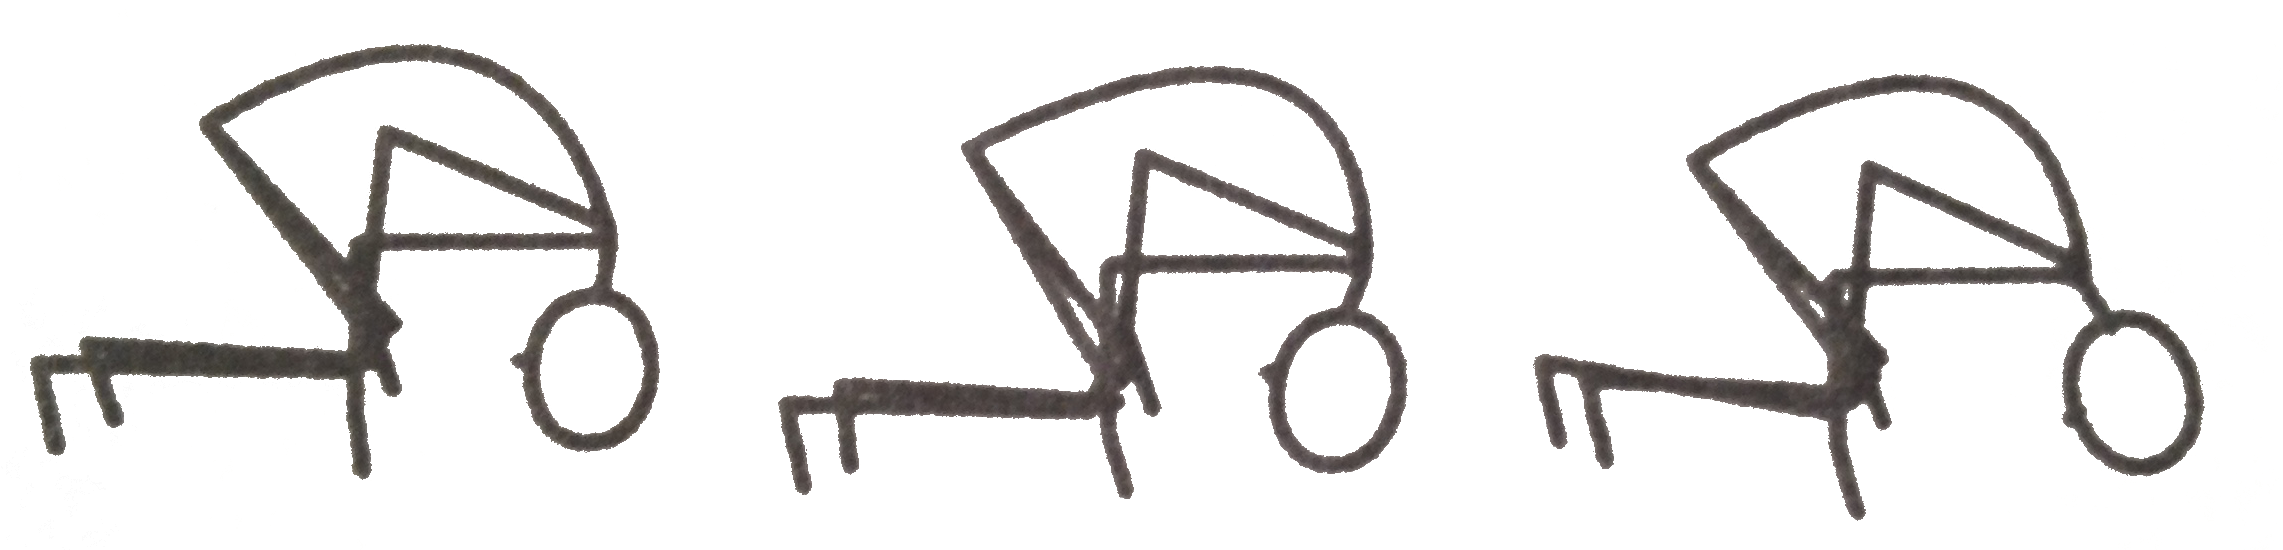
\includegraphics[width=1\linewidth]{HS_position.png}
%	\end{figure}

	\column{0.4\textwidth} % Left column and width
\structure{Kneel} down with your toes  tucked in and make a \structure{triangle with your hands and the head}, which is put on the ground with the crown, the highest point, touching the ground.                    

\structure{Roll your head gently} back and forwards.                                                                                                                                                                                                                                                                                                                                                                                                                                                                                                                                                                                                                                                                                                                                                                                                                                                                                                                                                                                                                                                                                                                                                                                                                                                                                                                                                                                                                                                                                                                                                                                                                                                                                                                                                                                                                                                                                                                                                                                                                                                                                                                                                                                                                                                                                                                                                                                                                                                                                                                                                                                                                                                                                                                                                                                                                                                                                                                                                                                                                                                                                                                                                                                                                                                                                                                                                                                                                                                                                                                                                                                                                                                                                                                                                                                                                                                                                                                                                                                                                                                                                                                                                                                                                                                                                                                                                                                                                                                                                                                                                                                                                                                                                                                                                                                                                                                                                                                                                                                                                                                                                                                                                                                                                                                                                                                                                                                                                                                                                                                                                                                                                                                                                                                                                                                                                                                                                                                                                                                                                                                                                                                                                                                                                                                                                                                                                                                                                                                                                                                                                                                                                                                                                                                                                                                                                                                                                                                                                                                                                                                                                                                                                                                                                                                                                                                                                                                                                                                                                                                                                                                                                                                                                                                                                                                                                                                                                                                                                                                                                                                                                                                                                                                                                                                                           
\end{columns}
\end{frame}
%---------------------------------------------------------------------------------

%-------------------------------------------------------------------
\begin{frame}
\frametitle{Shifting your weight}
\hypertarget{hemi}{}
\begin{columns}[c] % The "c" option specifies centered vertical alignment while the "t" option is used for top vertical alignment

\column{0.22\textwidth} % Left column and width
%	\begin{figure}
	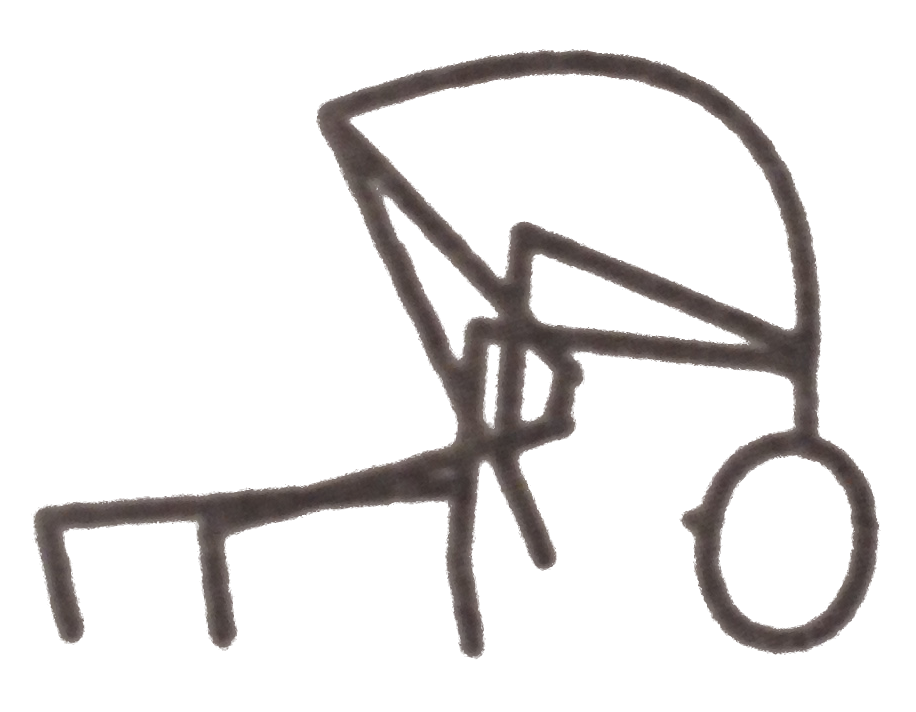
\includegraphics[width=1\linewidth]{HS_lift.png}
%	\end{figure}

	\column{0.4\textwidth} % Left column and width
\structure{Lift your knees} a bit off the ground. The pressure on the crown increases.

Try again in this position to \structure{roll} a bit forward and backwards. This will be way more difficult.                                                                                                                                                                                                                                                                                                                                                                                                                                                                                                                                                                                                                                                                                                                                                                                                                                                                                                                                                                                                                                                                                                                                                                                                                                                                                                                                                                                                                                                                                                                                                                                                                                                                                                                                                                                                                                                                                                                                                                                                                                                                                                                                                                                                                                                                                                                                                                                                                                                                                                                                                                                                                                                                                                                                                                                                                                                                                                                                                                                                                                                                                                                                                                                                                                                                                                                                                                                                                                                                                                                                                                                                                                                                                                                                                                                                                                                                                                                                                                                                                                                                                                                                                                                                                                                                                                                                                                                                                                                                                                                                                                                                                                                                                                                                                                                                                                                                                                                                                                                                                                                                                                                                                                                                                                                                                                                                                                                                                                                                                                                                                                                                                                                                                                                                                                                                                                                                                                                                                                                                                                                                                                                                                                                                                                                                                                                                                                                                                                                                                                                                                                                                                                                                                                                                                                                                                                                                                                                                                                                                                                                                                                                                                                                                                                                                                                                                                                                                                                                                                                                                                                                                                                                                                                                                                                                                                                                                                                                                                                                                                                                                                                                                                                                                                                                            
\end{columns}
\end{frame}
%---------------------------------------------------------------------------------
%-------------------------------------------------------------------
\begin{frame}
\frametitle{Lifting your legs}
\hypertarget{hemi}{}
\begin{columns}[c] % The "c" option specifies centered vertical alignment while the "t" option is used for top vertical alignment

\column{0.67\textwidth} % Left column and width
%	\begin{figure}
	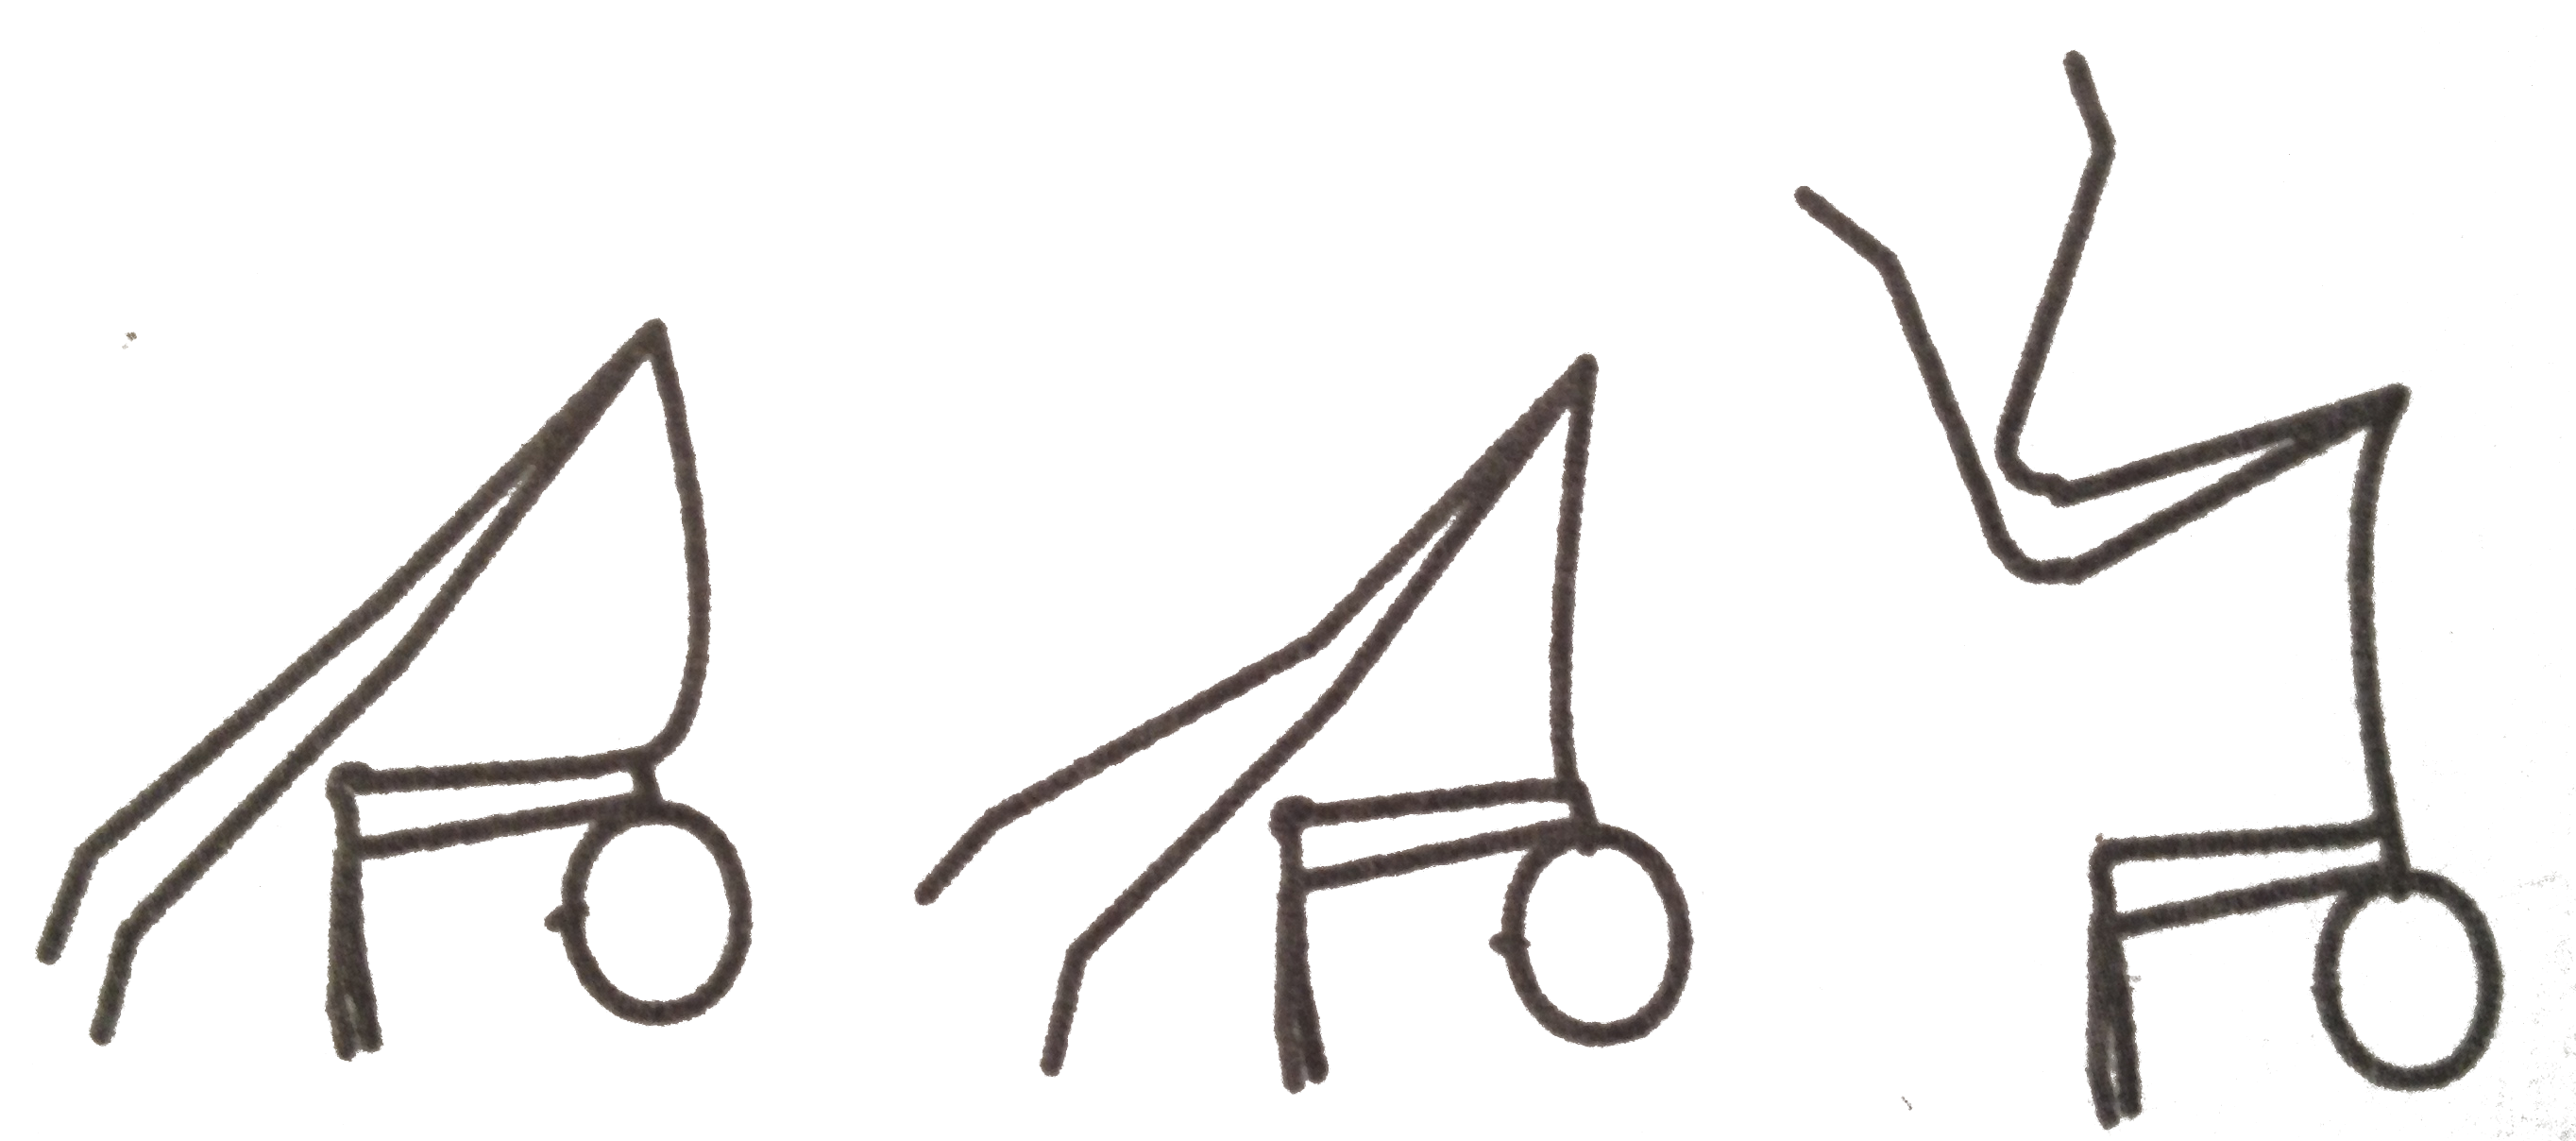
\includegraphics[width=1\linewidth]{HS_Upwards.png}
%	\end{figure}

	\column{0.33\textwidth} % Left column and width
\structure{Walk} with your \structure{feet} closer towards your head and push your \structure{backside towards ceiling}.

Try to bring your feet away from the ground by making a hollow back.

It's important to \structure{first bring the feet up}, not the  legs.                                                                                                                                                                                                                                                                                                                                                                                                                                                                                                                                                                                                                                                                                                                                                                                                                                                                                                                                                                                                                                                                                                                                                                                                                                                                                                                                                                                                                                                                                                                                                                                                                                                                                                                                                                                                                                                                                                                                                                                                                                                                                                                                                                                                                                                                                                                                                                                                                                                                                                                                                                                                                                                                                                                                                                                                                                                                                                                                                                                                                                                                                                                                                                                                                                                                                                                                                                                                                                                                                                                                                                                                                                                                                                                                                                                                                                                                                                                                                                                                                                                                                                                                                                                                                                                                                                                                                                                                                                                                                                                                                                                                                                                                                                                                                                                                                                                                                                                                                                                                                                                                                                                                                                                                                                                                                                                                                                                                                                                                                                                                                                                                                                                                                                                                                                                                                                                                                                                                                                                                                                                                                                                                                                                                                                                                                                                                                                                                                                                                                                                                                                                                                                                                                                                                                                                                                                                                                                                                                                                                                                                                                                                                                                                                                                                                                                                                                                                                                                                                                                                                                                                                                                                                                                                                                                                                                                                                                                                                                                                                                                                                                                                                                                                                                                                       
\end{columns}
\end{frame}
%---------------------------------------------------------------------------------
%-------------------------------------------------------------------
\begin{frame}
\frametitle{Legs up}
\hypertarget{hemi}{}
\begin{columns}[c] % The "c" option specifies centered vertical alignment while the "t" option is used for top vertical alignment

\column{0.33\textwidth} % Left column and width
%	\begin{figure}
	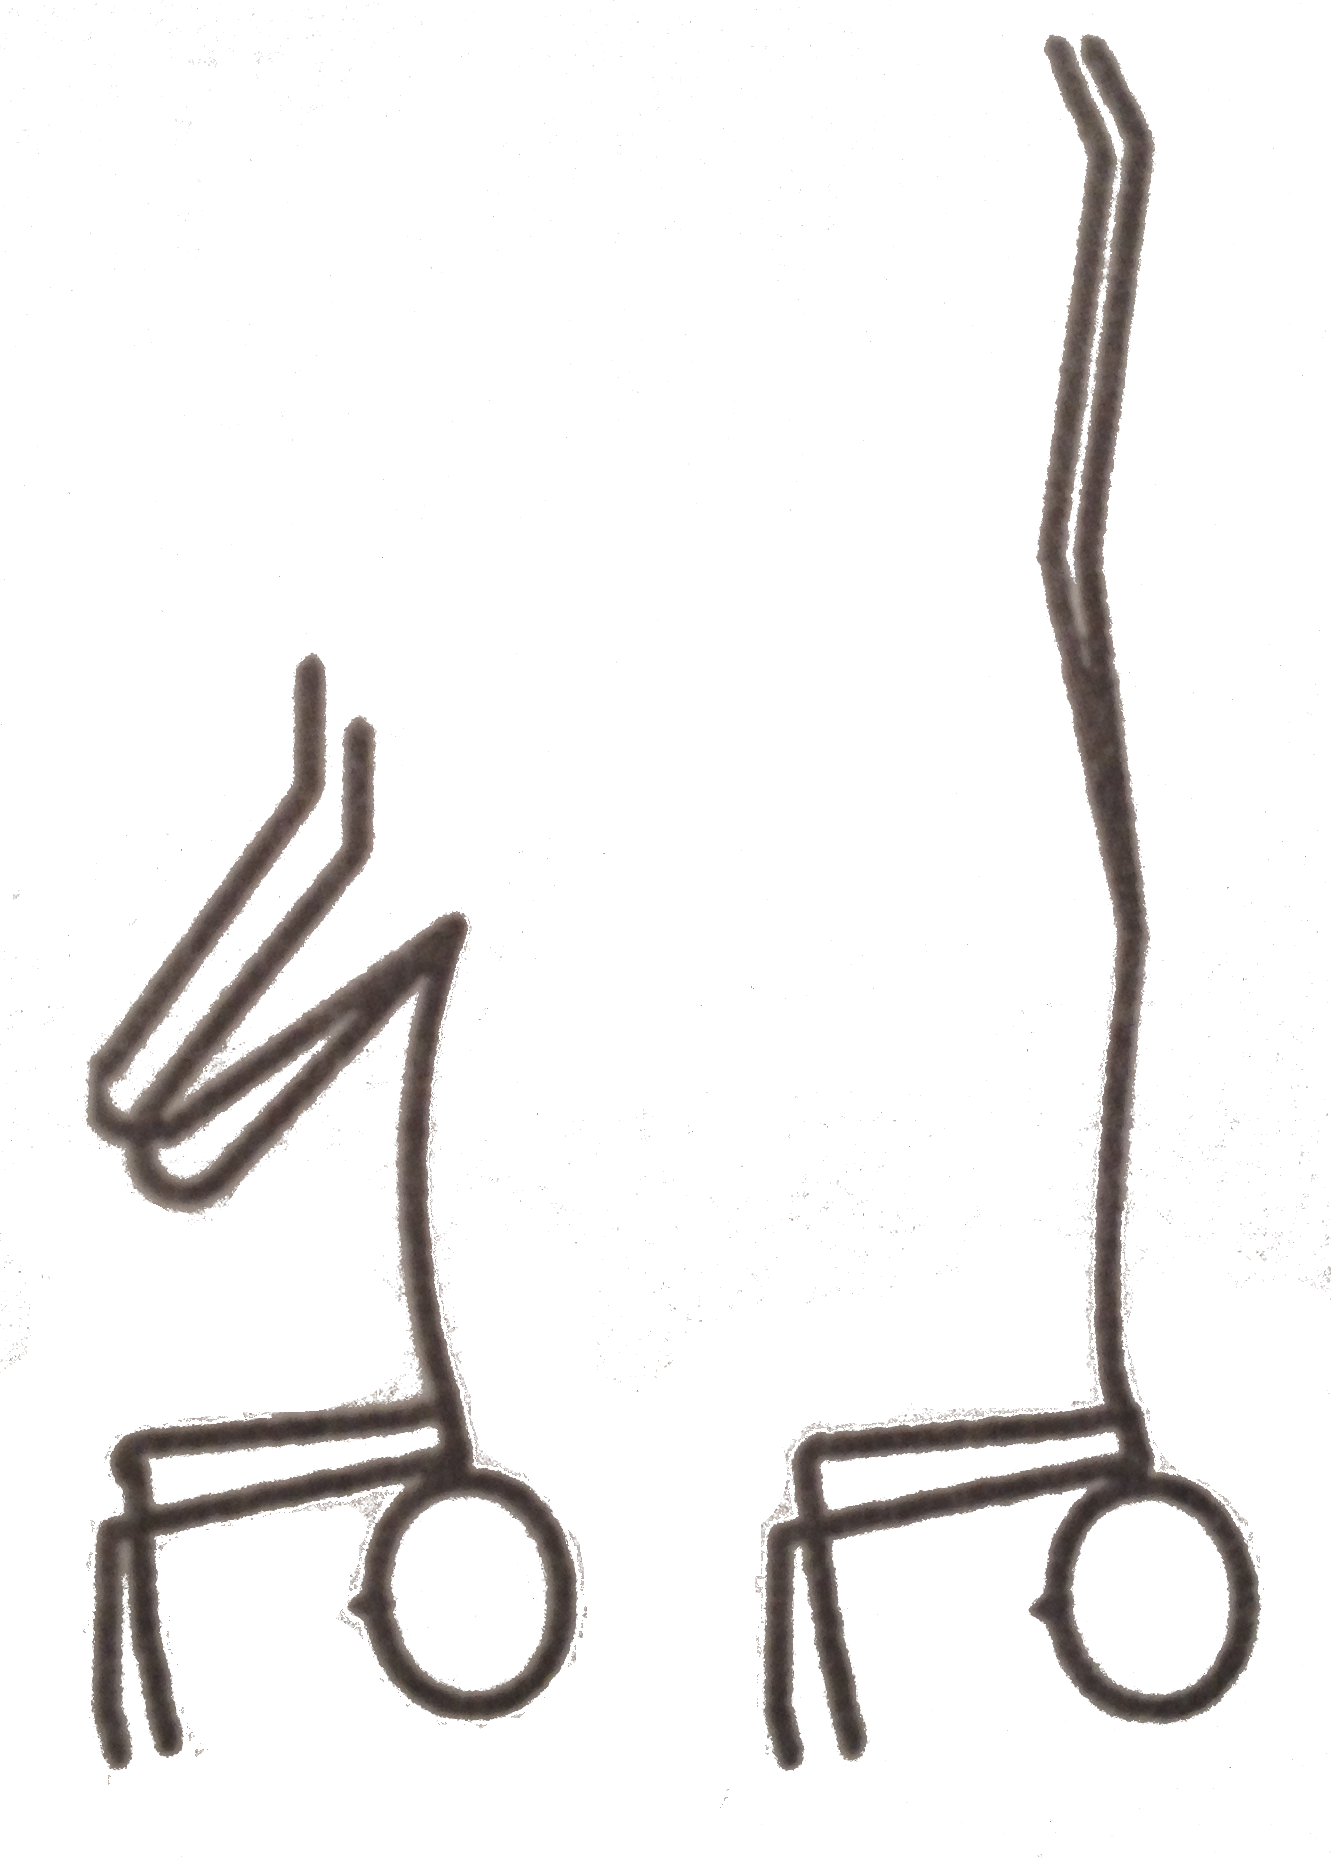
\includegraphics[width=1\linewidth]{HS_Up.png}
%	\end{figure}

	\column{0.5\textwidth} % Left column and width
Now pull your \structure{legs slowly up} with your hips. 

Let them \structure{first be tucked in} and only then \structure{slowly up} when you feel safe to do so.                                                                                                                                                                                                                                                                                                                                                                                                                                                                                                                                                                                                                                                                                                                                                                                                                                                                                                                                                                                                                                                                                                                                                                                                                                                                                                                                                                                                                                                                                                                                                                                                                                                                                                                                                                                                                                                                                                                                                                                                                                                                                                                                                                                                                                                                                                                                                                                                                                                                                                                                                                                                                                                                                                                                                                                                                                                                                                                                                                                                                                                                                                                                                                                                                                                                                                                                                                                                                                                                                                                                                                                                                                                                                                                                                                                                                                                                                                                                                                                                                                                                                                                                                                                                                                                                                                                                                                                                                                                                                                                                                                                                                                                                                                                                                                                                                                                                                                                                                                                                                                                                                                                                                                                                                                                                                                                                                                                                                                                                                                                                                                                                                                                                                                                                                                                                                                                                                                                                                                                                                                                                                                                                                                                                                                                                                                                                                                                                                                                                                                                                                                                                                                                                                                                                                                                                                                                                                                                                                                                                                                                                                                                                                                                                                                                                                                                                                                                                                                                                                                                                                                                                                                                                                                                                                                                                                                                                                                                                                                                                                                                                                                                                                                                                                                                   
\end{columns}

\vspace{1cm}
Back to \href{run:./Exercises.pdf}{\underline{exercises}}.
\end{frame}
%---------------------------------------------------------------------------------


\end{document} 